%----------------------------------------------------------------------------------------
%	PROGETTAZIONE
%----------------------------------------------------------------------------------------

\section{Progettazione}
Il processo di sviluppo adottato ha visto due fasi di progettazione ben distinte: il design architetturale e il design di dettaglio.\\ 

\subsection{Design Architetturale}

Dapprima il gruppo si è concentrato sul design architetturale, ovvero la definizione dell'architettura generale del sistema, delle sue componenti principali e delle relazioni tra di esse.\\
Ciò ha permesso di individuare fin da subito gli elementi più importanti del sistema e di definire le interfacce tra di essi, nonchè di scegliere le tecnologie più appropriate
per supportare il core del sistema.\\

Fin dalle prime fasi di analisi sono emersi due domini distinti ma connessi tra di loro:
\begin{itemize}
    \item \textbf{User Domain}: comprende tutti i componenti del sistema che concorrono a fornire un'interfaccia di accesso al sistema all'utente finale.
    \item \textbf{Charging Station Domain}: comprende tutti i componenti del sistema che concorrono a modellare il comportamento delle Charging Station e di monitornarne costantemente lo stato.
\end{itemize}

In seguito all'individuazione di questi domini, il gruppo ha individuato per ognuno di essi le componenti principali, che verranno di seguito discusse. \\

Per quanto riguarda lo User Domain:
\begin{itemize}
    \item \textbf{User App}: applicativo utilizzato dall'utente finale, costituisce l'interfaccia principale con il sistema, permettendo di visualizzare i dati e di interagire con esso.
    \item \textbf{Auth Server}: servizio che permette di registrare ed autenticare gli utenti permettendo loro di accedere al sistema. \\
    \item \textbf{User DB}: database che contiene le informazioni sugli utenti registrati al sistema.
\end{itemize}

La User App, all'avvio, richiederà all'utente di autenticarsi o registrarsi e genererà una richiesta HTTP da inviare all'Auth Server. Quest'ultimo interrogherà il database per verificare l'esistenza
dell'utente o per crearne uno nuovo. In seguito alla riuscita di queste operazioni, l'utente avrà accesso alla User App e potrà interagire con il sistema.\\

Per quanto riguarda il Charging Station Domain:
\begin{itemize}
    \item \textbf{Charging Station}: componente hardware che permette di ricaricare le batterie dei veicoli elettrici.
    \item \textbf{Charging Station Actor}: componente software che gestisce la Charging Station, permettendo di monitorare lo stato della stessa e di interagire con essa.
    \item \textbf{Charging Station Provider}: componente software che osserva lo stato delle Charging Station e ne fornisce un'interfaccia di accesso.
    \item \textbf{Charging Station Service}: sotto componente del Charging Station Provider, permette di esporre l'interfaccia del Charging Station Provider attraverso una API REST. \\
\end{itemize}

Siccome i dati relativi alle Charging Station sono conosciuti ed utilizzati dal Charging Station Actor, il gruppo ha deciso di non creare al momento un Database per memorizzarli, ma di utilizzare un modello a scambio di messaggi per effettuare
query direttamente sui Charging Station Actors.\\

I vari Charging Station Actors dunque gestiscono in maniera indipendente le Charging Station, e comunicano in maniera peer-to-peer con il Charging Station Provider, il quale può sia essere notificato
dai Charging Station Actors di eventuali cambiamenti di stato, sia interrogato dalla User App per ottenere informazioni sullo stato delle Charging Station attraverso l'API REST esposta dal Charging Station Service.\\

L'architettura complessiva del sistema è dunque riassunta nel seguente diagramma:

\begin{figure}[htbp]
    \centering
    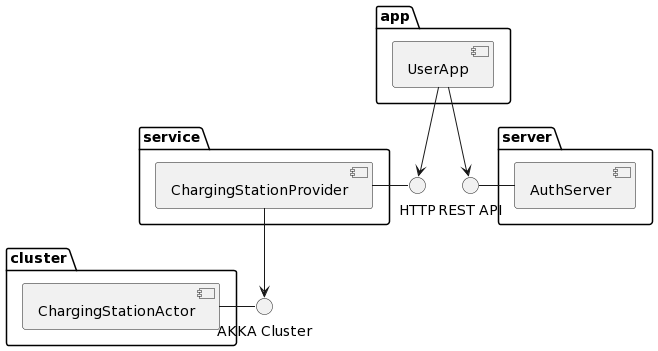
\includegraphics[width=\textwidth]{images/architecture.png}
    \caption{Diagramma dei Componenti per l'architettura del sistema}
    \label{fig:architecture}
\end{figure}

\subsection*{Design di Dettaglio}
TODO: spiega le interazioni tra gli attori e componenti del sistema, con descrizione sia testuale che con diagrammi di sequenza.\\


%Devono essere esposte le scelte progettuali operate nelle varie fasi di sviluppo dell'elaborato.\\

%In questa sezione devono essere documentati gli schemi di progetto relativamente all'architettura complessiva del sistema e alle sue componenti di rilievo che possano meritare un'analisi di dettaglio. Per le componenti software si può ricorrere ad esempio a diagrammi delle classi, di sequenza, stato, attività. Per le componenti hardware è possibile includere opportuni schemi in grado di descrivere l'architettura fisica adottata.\\

%Vincoli circa la lunghezza della sezione (escluse didascalie, tabelle, testo nelle immagini, schemi):

%\vspace{1cm}
%\begin{tabular}{l|rr}
% & Numero minimo di battute & Numero massimo di battute \\
% \hline
% 1 componente & 9000 & 18000 \\
% 2 componenti & 12000 & 21000 \\
% 3 componenti & 15000 & 24000 \\
% \hline
%\end{tabular}


\newpage